% LaTeX source for ``Introduction to Computer Science (Java/Pi Edition)''
% Copyright (c) 2015- David S. Read, All Rights Reserved

\chapter{Recursion}

\index{recursion}


\section{Divide and conquer}

\index{divide and conquer}
\index{algorithm!divide and conquer}

One approach that we may use when faced with a large task is to break it into smaller tasks, each a subset of the original large one. We work out each smaller task and in the process end up completing the larger one.

This process of expressing an algorithm by having it apply the same logic to a subset of the data is known as \textbf{recursion}.

Here are a couple of visual depictions of recursion. 

In this first image we see traditional \textit{Russian dolls}, where a set of dolls, each essentially a larger version of the previous, nest together to form the whole.\footnote{By Photo: RK812, Doll carved by Zvezdochkin, painted by Malyutin - Sergiev Posad Museum of Toys, Russia, Public Domain, https://commons.wikimedia.org/w/index.php?curid=5051554}

\beforefig
\centerline{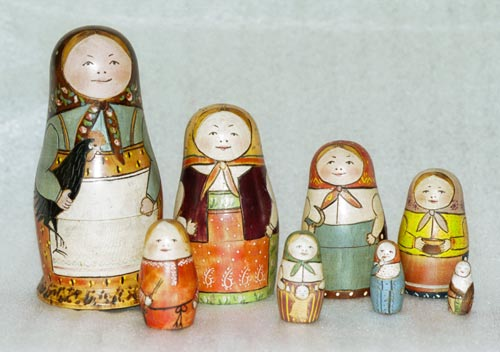
\includegraphics[height=2.5in]{images/recursion_First_matryoshka_museum_doll_open.jpg}}
\afterfig

In our second image, we see an artist painting a picture which shows an artist painting a smaller picture, which shows an artist painting a smaller picture...\footnote{Stack Exchange Network, http://programmers.stackexchange.com/questions/93826/how-do-i-explain-recursion-to-a-8-years-old-kid}

\beforefig
\centerline{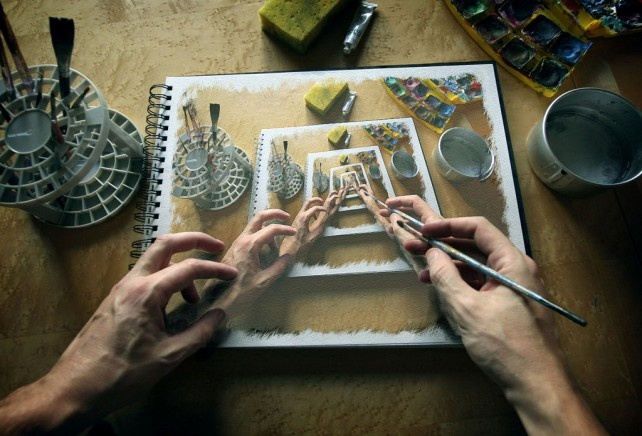
\includegraphics[height=2.5in]{images/recursion_quora.jpg}}
\afterfig

Both of these examples may help you understand recursion, however the images seem to be repeating the same information at different sizes. When we talk about using recursion in a computer program, it is the size of the data (meaning the values or the number of elements in an array) that is changing. In other words we are working with subsets, not duplicate information.

Here is an example of using recursion in the real world.\footnote{Quora, https://www.quora.com/How-should-I-explain-recursion-to-a-4-year-old} 

\begin{quotation}
The person behind you in a movie theater asks you what row you're sitting in. You don't want to count, so you ask the person in front of you what row they are sitting in, knowing that you will respond to the person behind you one greater than the answer the person in front of you gives. The person in front will ask the person in front of them. This will keep happening until the question reaches the front row, and it is easy to respond: "I'm in row 1!" From there, the correct message (incremented by one by the person in each row) will eventually make its way back to the person who asked.
\end{quotation}

\pagebreak

This exemplifies several key aspects of using recursion:
    
\begin{enumerate}
    \item The question ("what row am I in?") needs to be rephrased recursively as: "how many people are in front of me + 1?" with a base case of zero people in front of me (the front row).
    
    \item Considering the process of each person asking the person in front of them the same question, we can see that a recursive approach will work its way down to a base case (row 1 in this example) and then ``unwind'' back through all the recursive requests to return to the original requester who now has the answer.
    
    \item At each step, the process is the same, each requester has to add one to the answer from the person in front of them.
    
\end{enumerate}    
    
\section{Fibonacci sequence}    

Let's apply this concept in a mathematical context. One mathematical problem that is easily solved using a recursive approach is calculating Fibonacci numbers. As a refresher, the Fibonacci sequence starts out with the values 0 and 1. It then continues by adding the last two numbers of the current sequence to arrive at the next number in the sequence.

Specifically, starting with 0 and 1 as the sequence, we add them resulting in 1, which becomes the new end of the sequence. The last two numbers are now 1 and 1 which when added together are 2, which again becomes the last number in the sequence. The last two numbers are now 1 and 2 which sum to 3. This continues, 2 plus 3 is 5, 3 plus 5 is 8...

Here are the first 12 numbers in the Fibonacci sequence:

\beforeverb
\begin{verbatim}
0, 1, 1, 2, 3, 5, 8, 13, 21, 34, 55, 89
\end{verbatim}

Thinking about how this is calculated, we can break the problem down into a process of adding together the last two numbers in the current sequence, which in turn adds the previous last two numbers in the sequence, and continuing on until we have as much of the sequence as desired.

To create a method that is recursive we have to be sure to answer three questions, matching the key aspects we discussed in the movie theater row calculating example:

\begin{enumerate}
	\item What is the base case and how is the method written to identify it?
		
	\item What information does the recursive method need in order to calculate the new value?
	
	\item When is the process completed so that the method knows to stop recursing?
\end{enumerate}

In the case of the Fibonacci sequence we would answer those questions as follows:

\begin{enumerate}
	\item The base case is that the first value in the sequence is 0 and the second value in the sequence is 1.

	\item The method will need to add the last two numbers currently in the sequence if the base case does not apply.

	\item The method will need to be told which element of the sequence to compute.
\end{enumerate}

Here is how we could declare our \texttt{fibonacci} method, which accounts for the argument value we need (element number in the sequence we are to calculate):

\beforeverb
\begin{verbatim}
public int fibonacci(int sequencePosition) 
\end{verbatim}
\afterverb

Next we need to write the code to apply the base case. In other words, we know that the Fibonacci value for \texttt{sequencePosition} 0 is the value 0 and the Fibonacci value for \texttt{sequencePosition} 1 is the value 1:

\beforeverb
\begin{verbatim}
public int fibonacci(int sequencePosition) {
 if (sequencePosition == 0) {
  return 0;
 } else if (sequencePosition == 1) {
  return 1;
 }
}
\end{verbatim}
\afterverb

Finally we need to add the \textbf{recursive} part of the process. In this case we know that to compute the third value in the sequence we add the second and first values. For the fourth value we add the third and second values. More generally, for the \texttt{nth} value we add the \texttt{nth~-~1} and \texttt{nth~-~2} values. In code we would write the following to represent that logic:

\beforeverb
\begin{verbatim}
return fibonacci(sequencePosition - 1) 
      + fibonacci(sequencePosition - 2);
\end{verbatim}
\afterverb

What this says is that to calculate the Fibonacci value at a \texttt{sequencePosition} we will return the result of calling the \texttt{fibonacci} method passing \texttt{sequencePosition~-~1} and adding to that the value of calling the \texttt{fibonacci} method passing the value \texttt{sequencePosition~-~2}.

\pagebreak

Here is a complete version of a program implementing our recursive Fibonacci algorithm in a method called \texttt{fibonacci}. The \texttt{main} method calls the \texttt{fibonacci} method passing the value 4 to obtain and display the fifth value in the Fibonacci sequence\footnote{Remember sequence position 0 contains the first value.}:

\beforeverb
\begin{verbatim}
public class Fibonacci {
 public int fibonacci(int sequencePosition) {
  if (sequencePosition == 0) {
   return 0;
  } else if (sequencePosition == 1) {
   return 1;
  }

  return fibonacci(sequencePosition - 1)
            + fibonacci(sequencePosition - 2);
 }

 public static void main(String[] args) {
  Fibonacci gen = new Fibonacci();
  System.out.print(gen.fibonacci(4));
 }
}
\end{verbatim}
\afterverb

The program produces the following output:

\beforeverb
\begin{verbatim}
3
\end{verbatim}
\afterverb

This means that the fifth value in the Fibonacci sequence is the number 3, which is correct.

It may take some time studying and thinking through what is happening when the \texttt{fibonacci} method runs and calls itself to really grasp how this approach works.

One way to picture the code running is to imagine a stack of plates such as you might see at a salad bar. As new plates are added, the ones already there are pushed down. We call this a \textbf{Last-in, First-out} stack. The last plate added will be the first one removed. When we write recursive methods we are creating such a stack of values in the computer.

\index{stack}

When a method calls itself, the current set of parameters and local variables are "pushed down" and temporarily replaced by a new set of parameters and local variables which the recursive call uses. Once the recursive call ends, those original values are "popped up" and put back for the original method call to continue using.

Fundamentally, each call to a method creates its own unique set of parameters and local variables which are separate from the parameters and local variables used by any other calls to the same method. This happens for each call, so if we call a method 5 times there will be five independent sets of parameters and local variables created for that method.

Let's walk through the calculation of one value in the Fibonacci sequence using our \texttt{fibonacci} method and the concept of a stack. In this example we will look at what happens when we ask for the fifth value in the sequence, which, as we saw above, is 3.

We call the \texttt{fibonacci} method passing the number 4 as the \texttt{sequencePosition} argument.\footnote{We want the fifth value in the sequence. Remember the first value in the sequence is in the zero-eth position.} Inside the method this means that the parameter \texttt{sequencePosition} has the value 4. Looking at the logic in the \texttt{fibonacci} method, the two Boolean tests will be false (4 isn't 0 and it isn't 1) and we'll end up at the recursive statement:

\beforeverb
\begin{verbatim}
return fibonacci(sequencePosition - 1) 
         + fibonacci(sequencePosition - 2);
\end{verbatim}
\afterverb

This means that we will call the \texttt{fibonacci} method passing the value 3 \mbox{(e.g. 4-1)}. This is a recursive request, the method is calling itself. The currently executing copy of the \texttt{fibonacci} method (with \texttt{sequencePosition} = 4) will wait until it gets the answer back from its recursive calls.

We now start executing a new copy of \texttt{fibonacci} passing 3 as the value for \texttt{sequencePosition}. Again, we skip past the two Boolean tests and end up at the recursive call. We then recurse again, passing 2 as the value for \texttt{sequencePosition}. This new executing copy of the \texttt{fibonacci} method will wait until it gets the answer back from its recursive call. We now have two copies of the \texttt{fibonacci} method waiting on results from their recursive calls.

Eventually we'll end up calling \texttt{fibonacci} with the value 1, which is a base condition. In that case the method returns the number 1 back to its caller. This allows the previous executing copy of \texttt{fibonacci} to continue running, using the returned value. This process continues to unwind its way back to the top of the stack, which is the original call made to \texttt{fibonacci} in the \texttt{main} method.

Thinking back to the movie row example, this is similar to how each person asking the person in front of them for their row number has to wait for that person to get an answer from the person in front of them before they will respond to the person behind them. Eventually the request reaches a person in the front row who immediately responds ``1''.

\pagebreak

Here are two depictions of the entire recursive process for our Fibonacci example where we ask for the fifth element in the sequence. The first depiction illustrates the set of recursive calls showing the \texttt{sequencePosition} value being passed into the method with each call. The numbers in the circles depict the order in which these recursive calls occur when the program runs.

\beforefig
\centerline{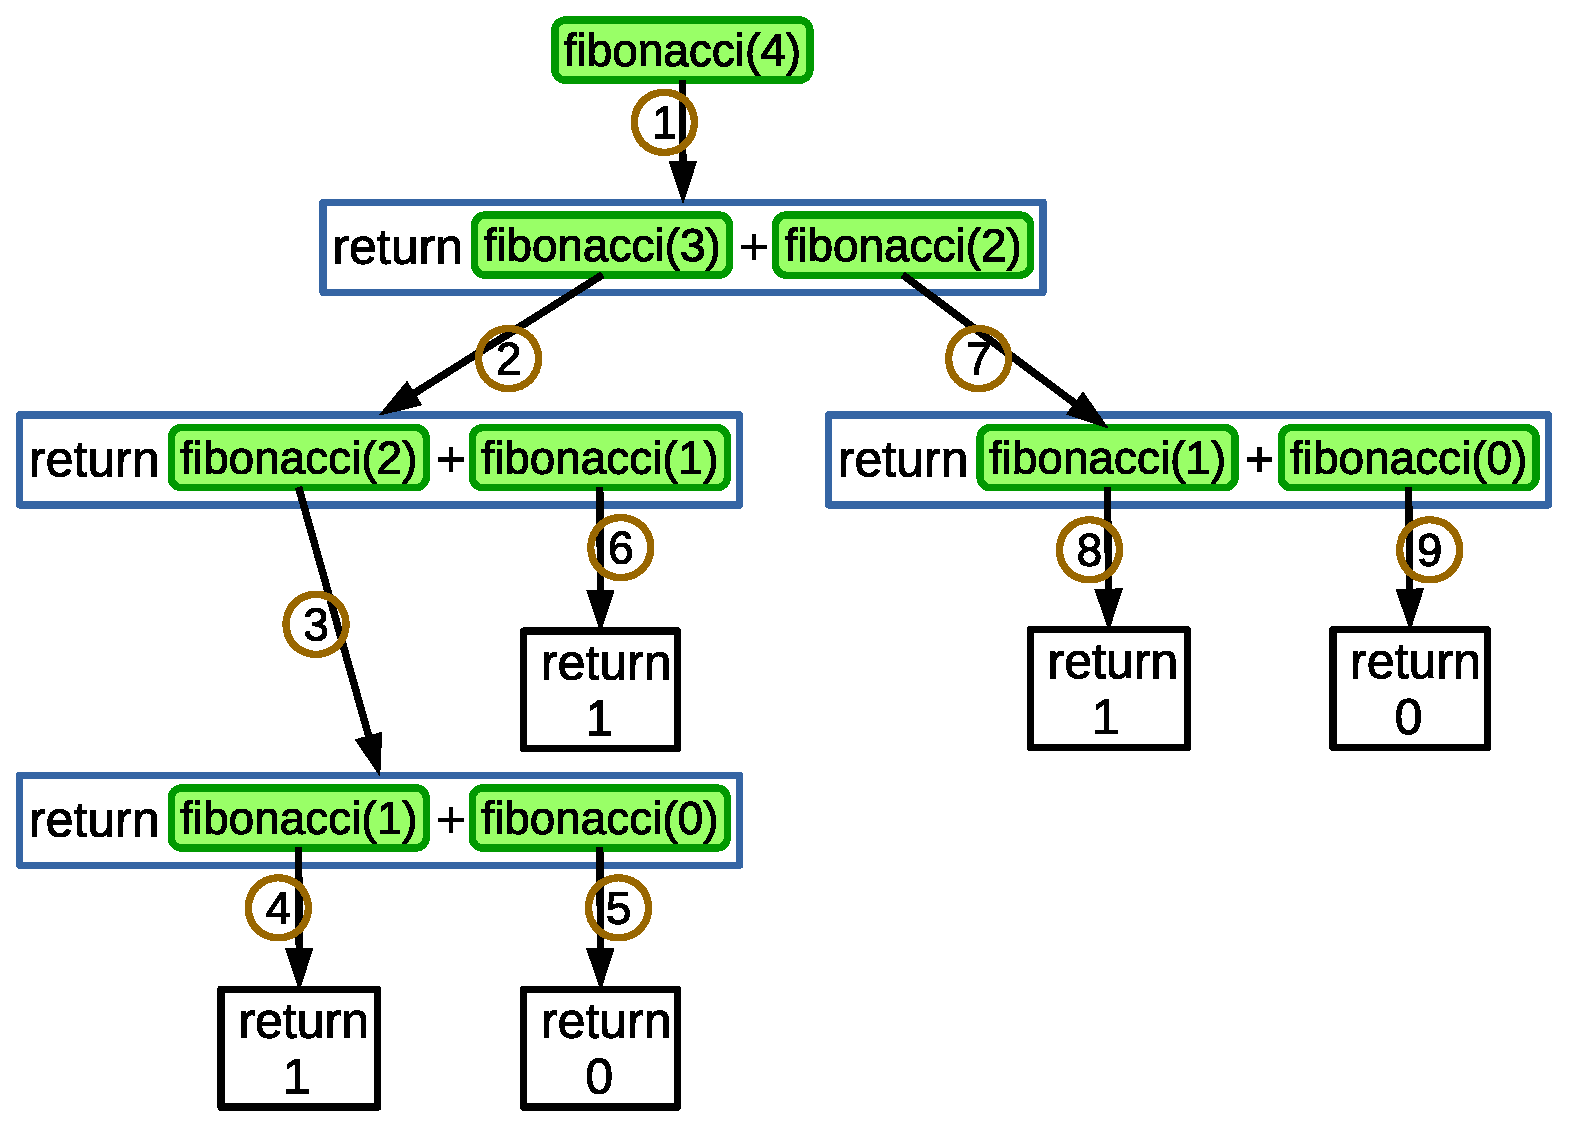
\includegraphics[height=2in]{figs2/recursion-fibonacci-depiction-0.eps}}
\afterfig

This next image depicts the value being returned by each call and the order in which those returns occur. You'll note that the initial call (where we pass in the argument 4 asking for number in the fifth position of the sequence) contains the number 3, which is the fifth number in the sequence. That is calculated based on the summing of the values from the recursive calls right below, which use the sums of values from the recursive calls below them.

\beforefig
\centerline{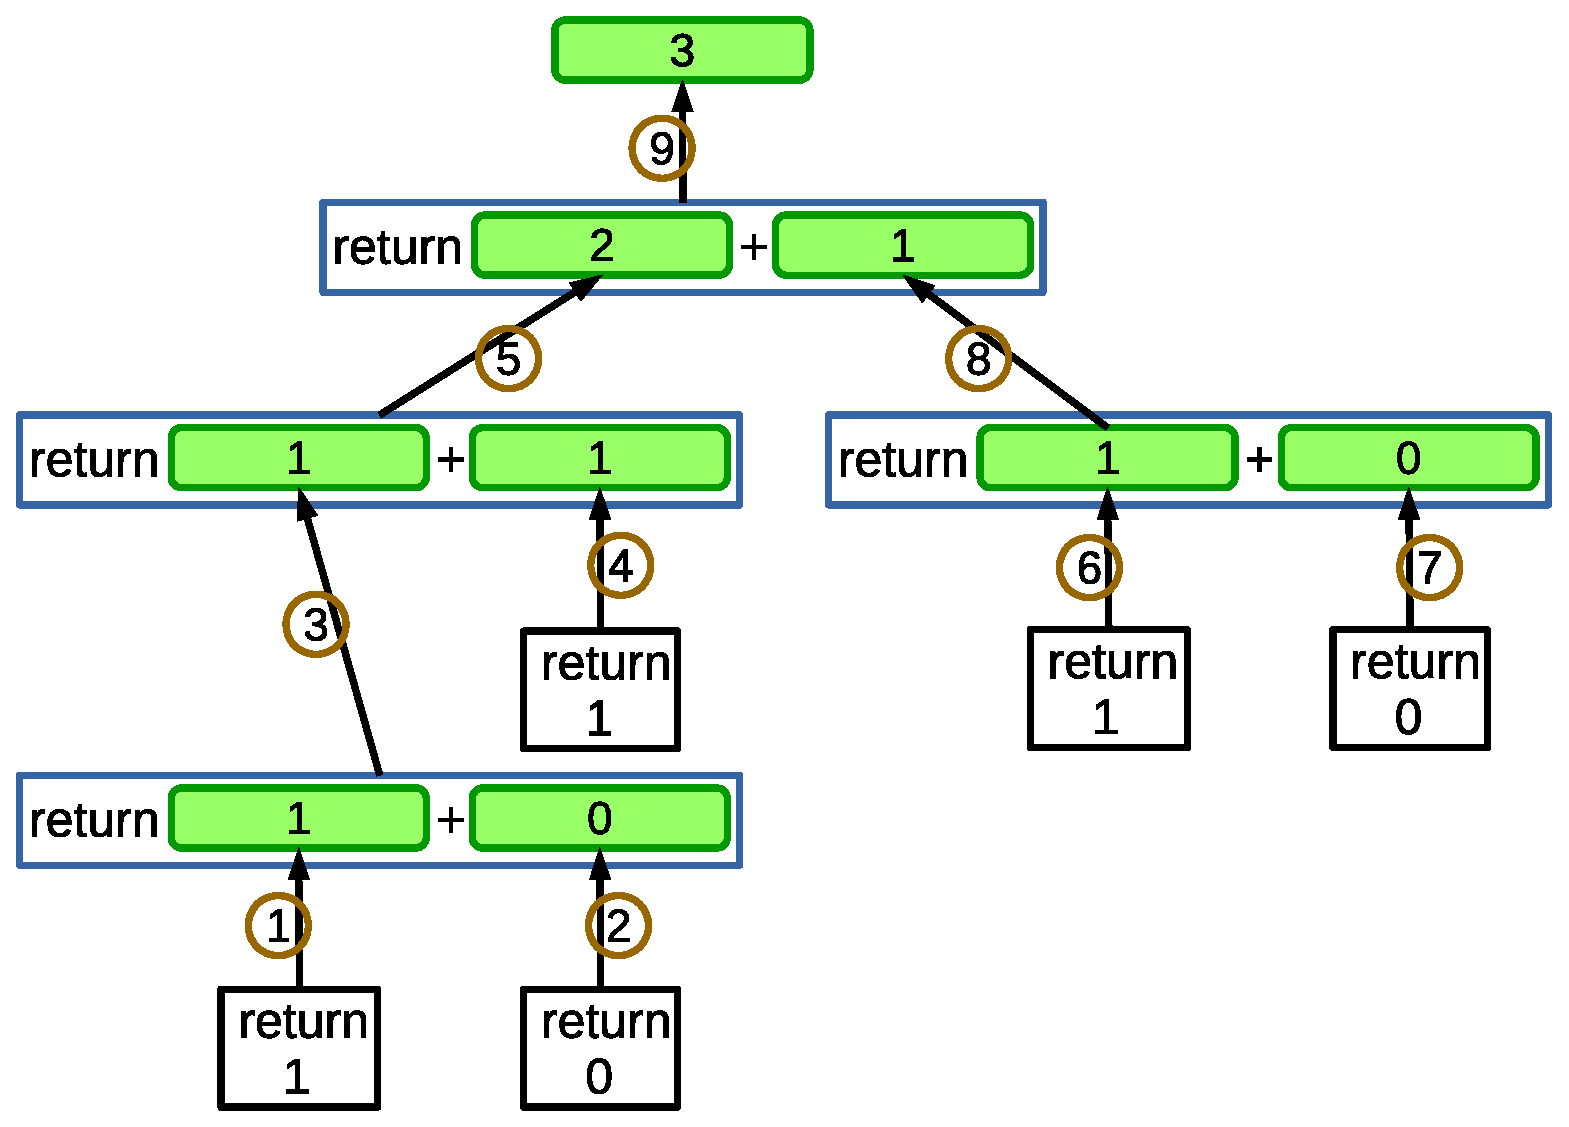
\includegraphics[height=2in]{figs2/recursion-fibonacci-depiction-1.eps}}
\afterfig

\section{Searching an ordered array}

Another example of a common recursive process is searching an ordered array for a specific value. For example, imagine we are creating a program to check the spelling of words. We already have an array of words that is stored in alphabetical order. Our program needs to accept a word from the user and tell him or her whether it is spelled correctly, or at least if it is a word that is in our array of words.

One way we could write the search would be to start at the beginning of the array and hunt through until we either find a match or arrive at the end of the array. If we find a match we can stop searching and tell the user that the word is spelled correctly. If we reach the end of the array we know the word isn't in our array and we tell the user we can't find that word.

This is a fairly inefficient approach to searching the array. If there are 1,000,000 (one million) words in the array, we will have to hunt through all million words in order to determine that a word is misspelled. If we wanted to use this to spell check a term paper, it would take a long time to run. Is there a better way?

Consider how you would do this task manually, perhaps using a dictionary. You would not start reading words at the beginning and go sequentially through until you matched the word or got to the end of the dictionary. Instead, what would you do? You would jump to the section of the dictionary that begins with the same letter that the word begins with. You would then jump several pages forward, check if the word was further on or earlier and jump forward or back in smaller and smaller increments as appropriate.

With this approach when are you done? Just like the earlier sequential approach, if you find a match you are done and you know the word is spelled correctly. What about the case where the word isn't in the dictionary? You know you are done when you find the location where the word would be if it were there. In other words, when you find two words next to each other where the first comes before the word you seek and the second comes after, you know that your word isn't present.

\section{Binary search}

To search this way using our ordered array example with a computer program we have to make one simplification to the process just described. As humans looking at a dictionary, which is generally organized to make jumping to a specific first letter easy, we can get to the correct part of the dictionary very fast. Our array, however, doesn't have a way to know where each set of words beginning with a specific letter starts. Instead we'll have the computer jump to the middle of the array and check for which of three conditions is true:

\begin{enumerate}
	\item The word in the middle of the array matches the word we are searching for
	\item The word in the middle of the array comes before (in alphabetical order) the word we are searching for
	\item The word in the middle of the array comes after the word we are searching for
\end{enumerate}

If the word is a match, we are done. We found the word and can return a result indicating the word is spelled correctly.

What about the other two cases? Based on our comparison with the word in the middle of the array we know whether the word we are searching for comes before or after the word at that location in the array.

We then logically divide the array into two parts, the set of words in the first half of the array and the set of words in the second half of the array. What we are creating are two \textbf{subarrays}, each containing half of the words that were in the original array. 

If the word we seek comes after the word we found in the middle of the original array then we know that our word, if it is present in the array at all, would have to be in the second subarray (remember the array is alphabetically ordered). In this case we do not need to look at the first subarray at all, our word can't be there.

We then treat that subarray as our array to be searched and repeat the process. We jump to the middle of that subarray and check to see which of the three conditions (listed above) are met.

In terms of set size, after our first comparison we have divided the number of words to be searched in half. After the second comparison we have reduced it to one-quarter. The third comparison reduces the amount of the array remaining to one-eighth of the original. You may notice a pattern here. With each comparison we are reducing the remaining amount of the array to search by a factor of 2 of what it was previously.

It turns out this approach of searching is amazingly efficient. In fact, to search our 1,000,000 words, the worst case number of comparisons is the square root of 1,000,000. That turns out to be 1,000. Remember though, the key to being able to do this is to have the array elements in ascending order. The name of this form of search is known as a \textbf{binary search}.

\index{binary search}

We use the term \textit{binary} for the search because it continually divides the remainder of the set in half, creating two subarrays. One subarray may hold a matching value and the other can be ignored.

How does this relate to recursion? Reviewing the process of a \textit{binary search} you'll note that it is carrying out the same operation on smaller subsets of the data. The operation always jumps to the middle of the remaining subarray, checks whether the value matches the one we seek or, if it doesn't match, figures out if the value would be earlier or later in the subarray.

The stop conditions are reached when either:

\begin{enumerate}
	\item A match is found
	\item The subdividing of the array has reduced down to a subset with one element and that element's value does not match the word we are seeking
\end{enumerate}

For this example, the information a recursive method would need includes the sorted array of words, the current start and end positions of the subarray being searched and the word being sought.

The method would check the center of the subarray for the word. If the method finds a match it is done and returns a success result, either a Boolean \texttt{true} or perhaps the array index location containing the word. 

If the word is not matched at the center of the subarray, the method will check whether the word is alphabetically greater or less than the word found in the middle of the array. It then makes a recursive call, replacing the beginning or ending value of the subarray with the location of the old center, offset by one. For example, if the word being sought is greater than the one found then the recursive call needs to check the elements from the old center plus one to the end of the subarray.

\section{Depicting a successful binary search}

Let's illustrate the process of a binary search without worrying about programming it yet. First, we'll work through a depiction of the process where the value we are searching for is in the array. 

For our example, we start with an array containing 10 fruit names in alphabetical order. In the image we see each word and to the left the element number in the array which contains that value. The array has 10 values so the array elements are numbered 0 to 9.

\beforefig
\centerline{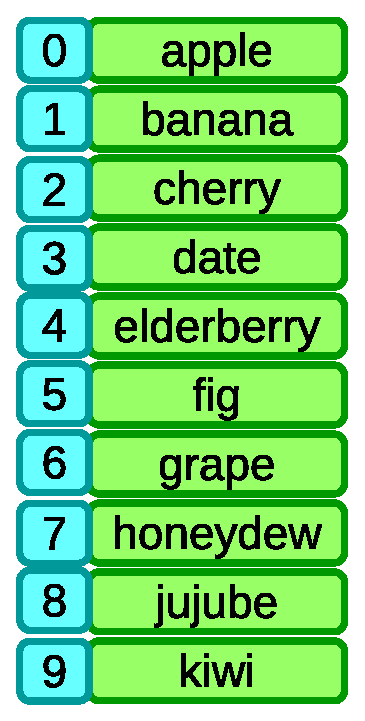
\includegraphics[height=2in]{figs2/recursion-binsearch-initiallist.eps}}
\afterfig

We want to see if the word \textbf{jujube} matches one of our words. We start by finding the middle of the array. To find the middle we add the starting index value to the ending index value and divide by 2. For this process we always use integer division (no fractional part). Given our 10 element array we calculate \texttt{(0 + 9) / 2} resulting in the integer value \texttt{4}. We compare our search term, \textbf{jujube}, to the word located in element 4, which is \textbf{elderberry}.

\beforefig
\centerline{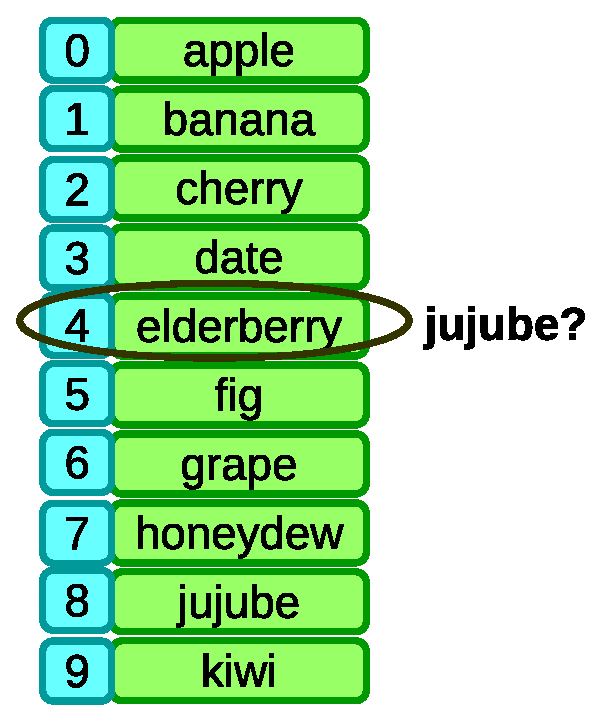
\includegraphics[height=2in]{figs2/recursion-binsearch-success-1.eps}}
\afterfig

The words do not match, so we check to see if \textbf{jujube} comes before or after \textbf{elderberry}. It comes after, meaning that if it is in the list it must be in an element further down the array. All the elements before the one containing \textbf{elderberry}, as well as the element containing \textbf{elderberry}, cannot contain our word and do not need to be looked at.

Since we know the word would come after the position just checked, we change the starting position to be one greater than the position just checked, which is the value  5.

\beforefig
\centerline{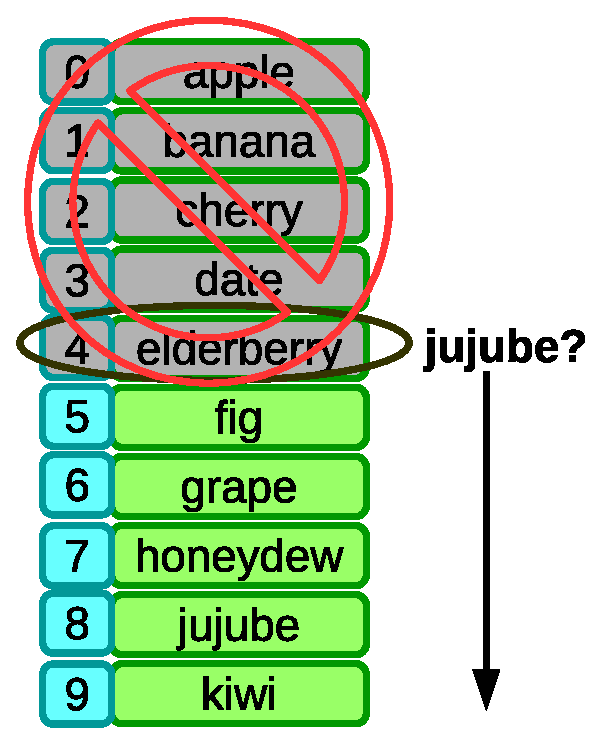
\includegraphics[height=2in]{figs2/recursion-binsearch-success-2.eps}}
\afterfig

Now we need to repeat this process on the remaining subarray. We calculate the middle element of the remaining elements. Our updated starting element number (as described above) is 5 (one past elderberry) and the end is still 9. Our calculation is then \texttt{(5 + 9) / 2} which results in \texttt{7}. We compare our search term, \textbf{jujube}, to the word located in element 7, which is \textbf{honeydew}.

\beforefig
\centerline{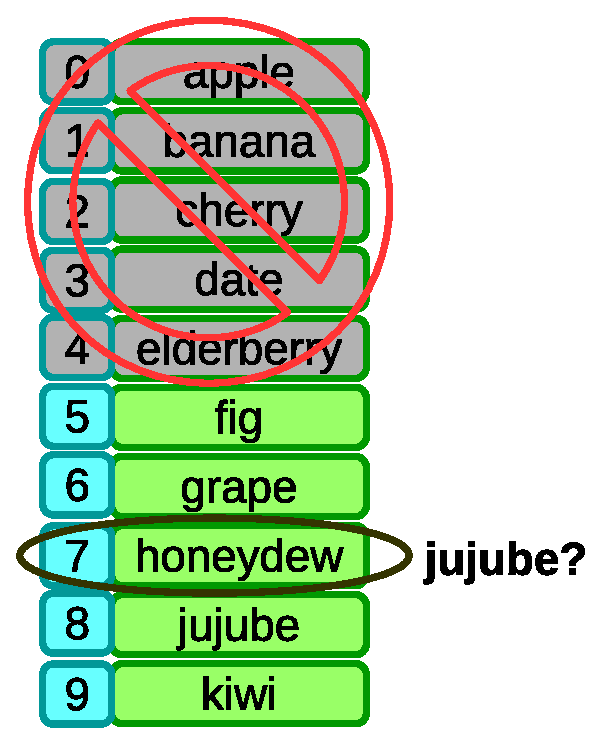
\includegraphics[height=2in]{figs2/recursion-binsearch-success-3.eps}}
\afterfig

The words do not match, so we check to see if \textbf{jujube} comes before or after \textbf{honeydew}. It comes after, meaning that if it is in the list it must be in an element further down the array. All the elements before the one containing \textbf{honeydew}, as well as the element containing \textbf{honeydew} cannot contain our word and do not need to be looked at.

Since we know the word would come after the position just checked, we again change the starting position to be one greater than the position just checked, which is the value  8.

\beforefig
\centerline{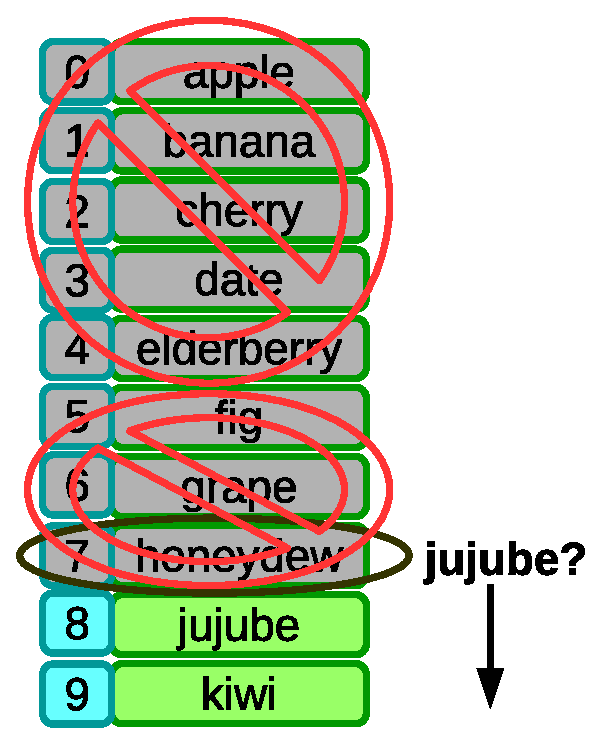
\includegraphics[height=2in]{figs2/recursion-binsearch-success-4.eps}}
\afterfig

Again we repeat this process on the remaining subarray. We calculate the middle element of the remaining elements. Our new starting element number is 8 and the end is still 9. Our calculation is then \texttt{(8 + 9) / 2} which results in \texttt{8}. We compare our search term, \textbf{jujube}, to the word located in element 8, which is \textbf{jujube}.

\beforefig
\centerline{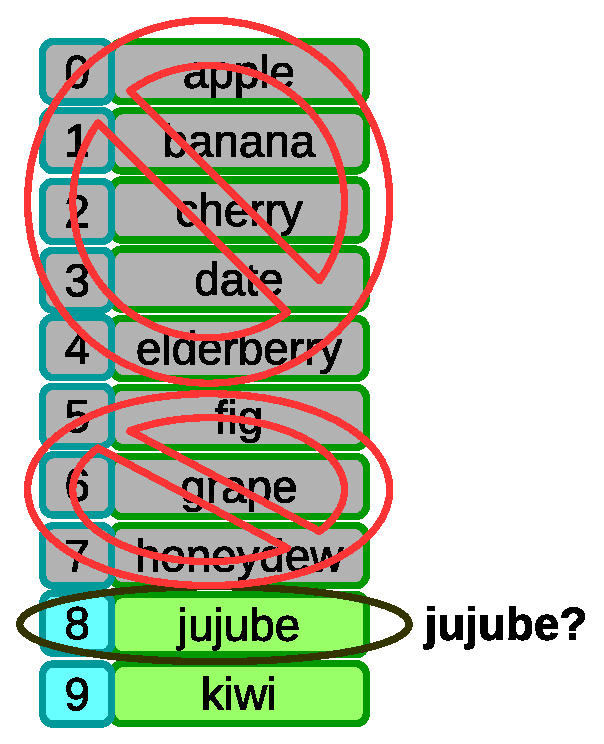
\includegraphics[height=2in]{figs2/recursion-binsearch-success-5.eps}}
\afterfig

The words match! The search is completed having made only 3 comparisons in our list of 10 elements.

\beforefig
\centerline{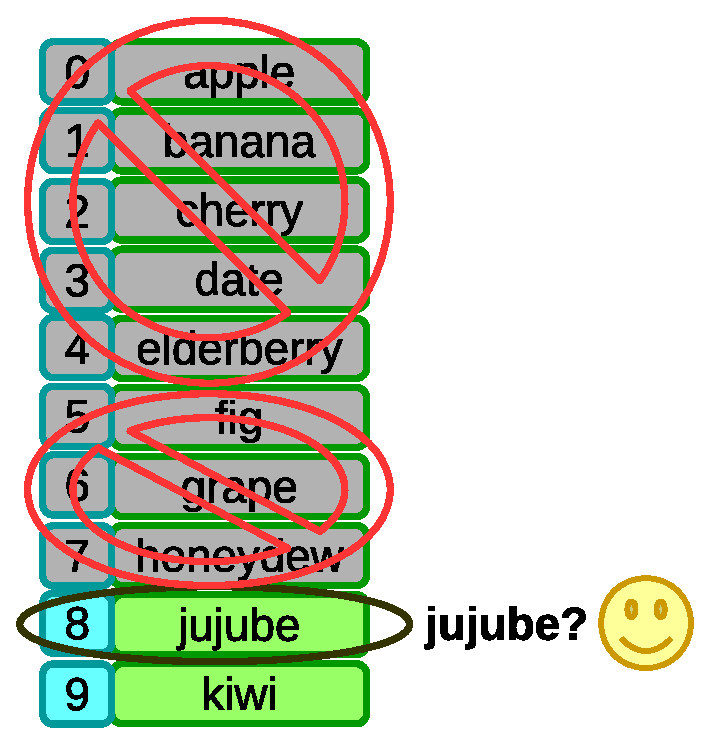
\includegraphics[height=2in]{figs2/recursion-binsearch-success-6.eps}}
\afterfig

\section{Depicting an unsuccessful binary search}

Here is a depiction of the binary search process where the value we are searching for is \textit{not} in the array. We start with the same array of 10 fruit names in alphabetical order. 

\beforefig
\centerline{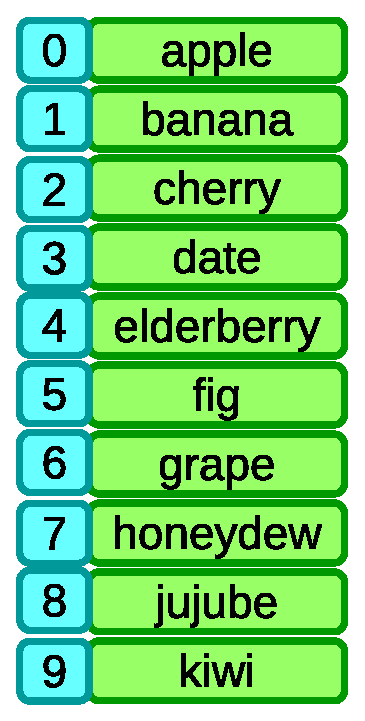
\includegraphics[height=2in]{figs2/recursion-binsearch-initiallist.eps}}
\afterfig

We want to see if the word \textbf{celery} matches one of our words. As before, we start by finding the middle of the array, element 4. We compare our search term, \textbf{celery}, to the word located in element 4, which is \textbf{elderberry}.

\beforefig
\centerline{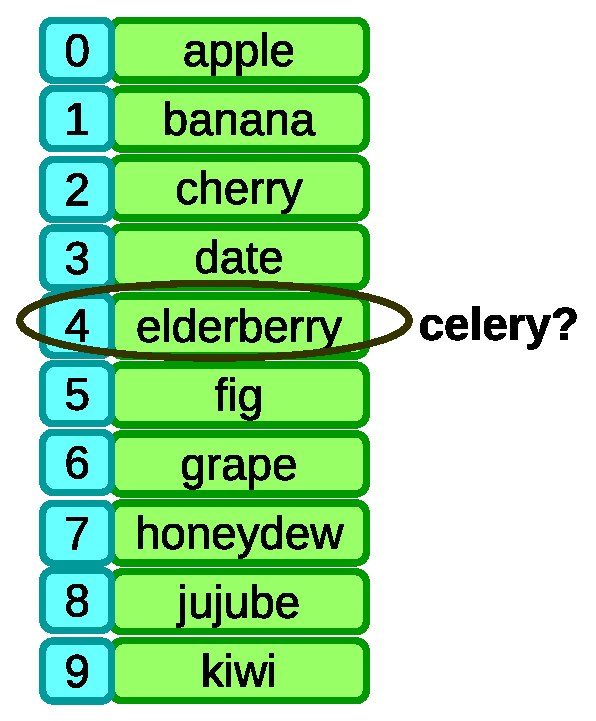
\includegraphics[height=2in]{figs2/recursion-binsearch-failure-1.eps}}
\afterfig

The words do not match, so we check to see if \textbf{celery} comes before or after \textbf{elderberry}. It comes before, meaning that if it is in the list it must be in an element earlier in the array. All the elements after the one containing \textbf{elderberry}, as well as the element containing \textbf{elderberry}, cannot contain our word and do not need to be looked at.

Since we know the word would come before the position just checked, we change the ending position to be one less than the position just checked, which is the value 3.

\beforefig
\centerline{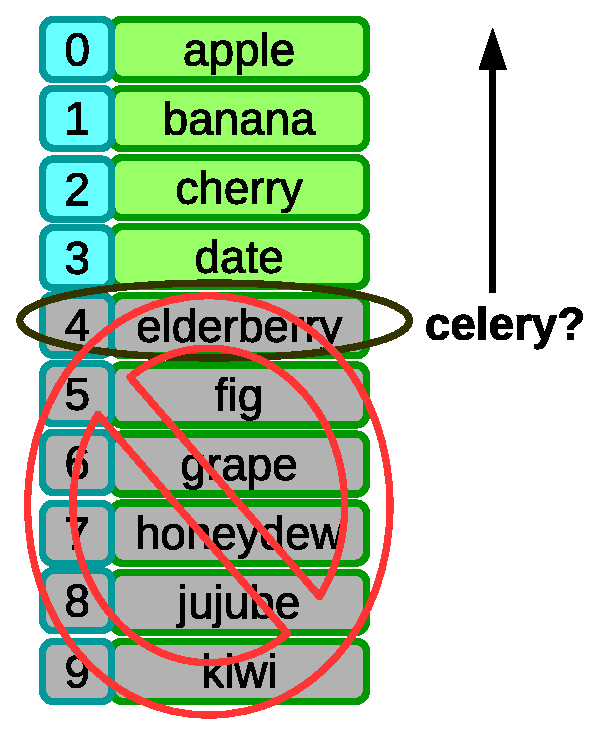
\includegraphics[height=2in]{figs2/recursion-binsearch-failure-2.eps}}
\afterfig

Again, we need to repeat this process on the remaining subarray. We calculate the middle element of the remaining elements. Our updated ending element number (as descrbied above) is 3 (one before elderberry) and the beginning is still 0. Our calculation is then \texttt{(0 + 3) / 2} which results in \texttt{1}. We compare our search term, \textbf{celery}, to the word located in element 1, which is \textbf{banana}.

\beforefig
\centerline{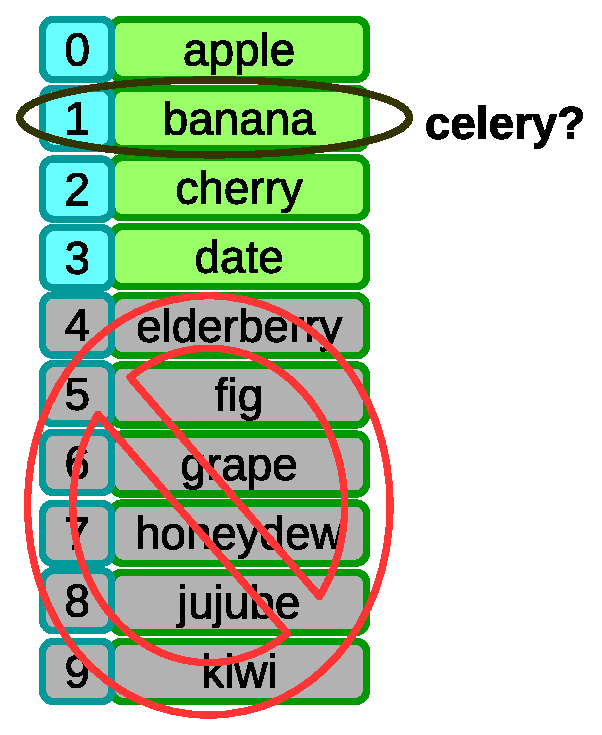
\includegraphics[height=2in]{figs2/recursion-binsearch-failure-3.eps}}
\afterfig

The words do not match, so we check to see if \textbf{celery} comes before or after \textbf{banana}. It comes after, meaning that if it is in the list it must be in an element further down the array. All the elements before the one containing \textbf{banana}, as well as the element containing \textbf{banana} cannot contain our word and do not need to be looked at.

Since we know the word would come after the position just checked, we change the starting position to be one greater than the position just checked, which is the value 2.

\beforefig
\centerline{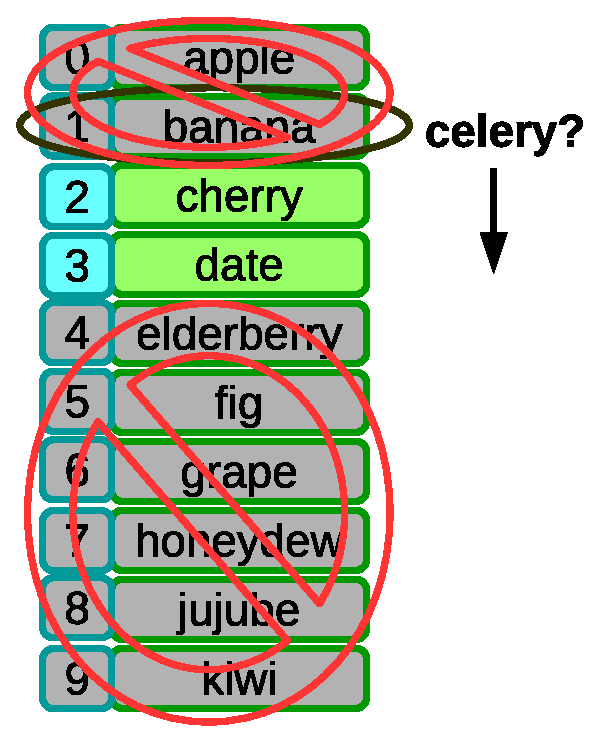
\includegraphics[height=2in]{figs2/recursion-binsearch-failure-4.eps}}
\afterfig

As usual, we repeat the process on the remaining subarray. We calculate the middle element of the remaining elements. Our updated starting element number is 2 and the end is still 3. Our calculation is then \texttt{(2 + 3) / 2} which results in \texttt{2}. We compare our search term, \textbf{celery}, to the word located in element 2, which is \textbf{cherry}.

\beforefig
\centerline{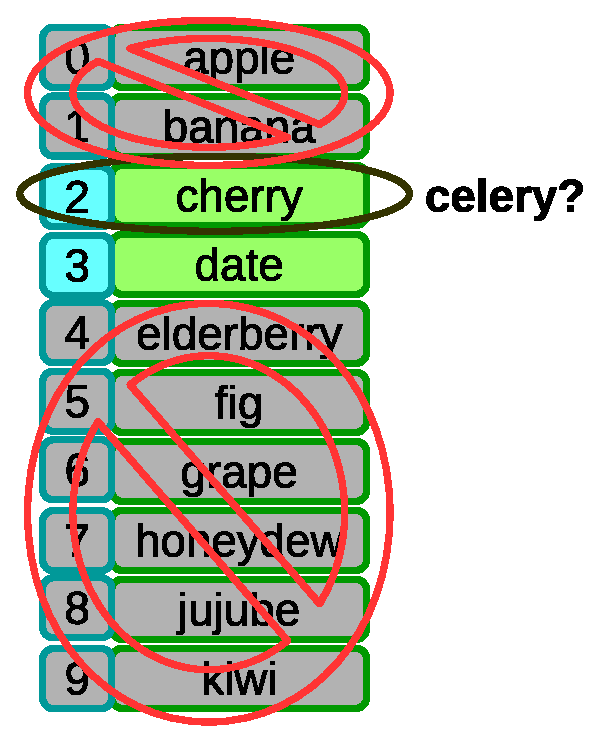
\includegraphics[height=2in]{figs2/recursion-binsearch-failure-5.eps}}
\afterfig

The words do not match, so we check to see if \textbf{celery} comes before or after \textbf{cherry}. It comes before, meaning that if it is in the list it must be in an element earlier in the array. 

Since we know the word would come before the position just checked, we change the ending position to be one less than the position just checked, which is the value 1. 

\beforefig
\centerline{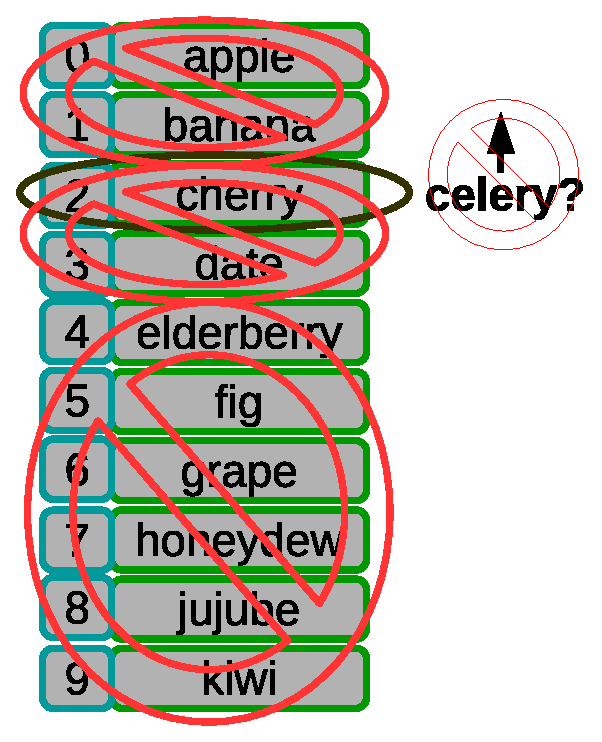
\includegraphics[height=2in]{figs2/recursion-binsearch-failure-6.eps}}
\afterfig

We now find that the starting element position is 2 and the ending element position 1. Since start is greater than end we know the word can't be in the array. 

Fundamentally, \textbf{\textit{all the earlier elements and all the later elements have been ruled out}}. Therefore the word must not be in the list. We have completed the search having made only 3 comparisons in our list of 10 elements.

\section{Implementing a recursive binary search}

Let's look at the code to implement the binary search process we just described. We'll call our class \texttt{WordSearch} and create a recursive method called \texttt{binarySearch} to implement the logic.

\index{recursive method}

There are four pieces of information the method needs:

\begin{enumerate}
	\item The ordered array of words
	\item The word we are searching for
	\item The current starting array element number
	\item The current ending array element number
\end{enumerate}

In the binary search process we will first calculate the center element. We will also need a variable to house the result of comparing the word being sought to the word in the center element of the subarray.

Next we need to compare the words (strings). Java has a string comparison method \texttt{compareToIgnoreCase()} which is perfect for our purposes. It will return 0 (zero) if the words match, a negative number if the word comes before the word being compared and a positive number if the word comes after the word being compared.

\index{compareToIgnoreCase}

For example, the Java code:

\beforeverb
\begin{verbatim}
int comparison = "Grape".compareToIgnoreCase("Apple");
System.out.println(comparison);
\end{verbatim}
\afterverb

Would output the value:

\beforeverb
\begin{verbatim}
6
\end{verbatim}
\afterverb

This means that the word \textit{Grape} comes after (alphabetically) the word \textit{Apple}. We don't need to be concerned with the specific value of 6. All that matters to us in this case is that if the number is greater than 0, the word comes after the word being compared and if it is negative the word comes before the word being compared.\footnote{If you are curious, the value returned is the lexical distance between the first unique letters encountered in the words. In this case the letter 'G' is 6 letters greater than the letter 'A'.}

The next part of the method will need to evaluate the result of the comparison, which we'll store in a variable called \texttt{comparison}. 

\begin{enumerate}
	\item If the value is 0 then we have found a match and we'll return the array index position of the element containing the word. 
	\item If the value is less than 0 we will update the ending array element number to be one less than the current center position (e.g. we know the word has to be earlier in the array).
	\item If the value is greater than 0 we will update the starting array element number to be one more than the current center position (e.g. we know the word has to be later in the array).
\end{enumerate}

Finally we need to determine whether we have reached the end of the process, meaning there is no smaller subset of the original array left to search. The easiest way to figure that out is to compare the updated start and end positions. If they cross, meaning that the start position becomes greater than the end position, we have finished the search and not found a match. If the start position is equal to or less than the end position we need to recurse and check the new subarray.

Here is the entire method, which implements the process just described. Make sure that each part makes sense and that you can see how the code relates to the explanation above.

\beforeverb
\begin{verbatim}
public class WordSearchNoTracing {
 private int binarySearch(String[] wordList, String searchTerm,
                                      int startPos, int endPos) {
  int checkPosition = (startPos + endPos) / 2;
  int comparison;

  // Compare the search term to the word in the center element of the
  // subarray
  comparison = searchTerm.compareToIgnoreCase(wordList[checkPosition]);

  if (comparison == 0) {
   // The words matched - return the matching position in the array
   return checkPosition;
  } else if (comparison < 0) {
   // The search term comes earlier in the array, change the ending
   // position
   endPos = checkPosition - 1;
  } else {
   // The search term comes later in the array, change the beginning
   // position
   startPos = checkPosition + 1;
  }

  // Check that there are still words left to check
  if (startPos <= endPos) {
   // Make a recursive call to search the new subarray
   return binarySearch(wordList, searchTerm, startPos, endPos);
  } else {
   // If the set was reduced to a single element with no match then the
   // word is not present
   return -1;
  }
 }

 public static void main(String[] args) {
  String[] fruits = { "apple", "banana", "cherry", "date", "elderberry", "fig",
      "grape", "honeydew", "jujube", "kiwi" };
  WordSearchNoTracing instance = new WordSearchNoTracing();

  int foundPosition = instance.binarySearch(fruits, "jujube", 0, fruits.length - 1);
  System.out.println("Find jujube? " + foundPosition);

  System.out.println("=============================");
  
  foundPosition = instance.binarySearch(fruits, "carrot", 0, fruits.length - 1);
  System.out.println("Find carrot? " + foundPosition);
 }
}
\end{verbatim}
\afterverb

When we run this we see the following output:

\beforeverb
\begin{verbatim}
Find jujube? 8
=============================
Find carrot? -1
\end{verbatim}
\afterverb

This means that \textit{jujube} was found in element 8 of the \texttt{fruits} array and \textit{carrot} was not found in the array (we chose to use -1 as the signal for not finding a match).

Let's add a few print statements so that we can see what is happening when the \texttt{binarySearch} method runs. Here is an updated version that includes some \texttt{System.out.println} calls to display the internal values as the recursive calls are made. 


\beforeverb
\begin{verbatim}
public class WordSearch {
 private int binarySearch(String[] wordList, String searchTerm, 
                                      int startPos, int endPos) {
  int checkPosition = (startPos + endPos) / 2;
  int comparison;

  System.out.println(
    "BinarySearch called for searchTerm:" + searchTerm + " 
               startPos:" + startPos + " endPos:" + endPos);

  // Compare the search term to the word in the center element of the
  // subarray
  comparison = searchTerm.compareToIgnoreCase(wordList[checkPosition]);

  System.out.println("checkPosition:" + checkPosition +
       " WordAtPosition:" + wordList[checkPosition] + 
       " comparison:" + comparison);

  if (comparison == 0) {
   // The words matched - return the matching position in the array
   System.out.println("Words matched at checkPosition: " + checkPosition);
   System.out.println();
   return checkPosition;
  } else if (comparison < 0) {
   // The search term comes earlier in the array, change the ending
   // position
   endPos = checkPosition - 1;
  } else {
   // The search term comes later in the array, change the beginning
   // position
   startPos = checkPosition + 1;
  }

  // Check that there are still words left to check
  if (startPos <= endPos) {
   // Make a recursive call to search the new subarray
   System.out.println("Make a recursive call. startPos:" + 
                             startPos + " endPos:" + endPos);
   System.out.println();
   return binarySearch(wordList, searchTerm, startPos, endPos);
  } else {
   // If the set was reduced to a single element with no match then the
   // word is not present
   System.out.println("No more elements to be searched. startPos:" + 
                                       startPos + " endPos:" + endPos);
   System.out.println();
   return -1;
  }
 }

 public static void main(String[] args) {
  String[] fruits = { "apple", "banana", "cherry", "date", "elderberry", "fig",
      "grape", "honeydew", "jujube", "kiwi" };
  WordSearch instance = new WordSearch();

  int foundPosition = instance.binarySearch(fruits, "jujube", 0, fruits.length - 1);
  System.out.println("Find jujube? " + foundPosition);

  System.out.println("=============================");

  foundPosition = instance.binarySearch(fruits, "carrot", 0, fruits.length - 1);
  System.out.println("Find carrot? " + foundPosition);
 }
}
\end{verbatim}
\afterverb

When we run this we see some details about how the recursive calls are operating:

\beforeverb
\begin{verbatim}
BinarySearch called for searchTerm:jujube startPos:0 endPos:9
checkPosition:4 WordAtPosition:elderberry comparison:5
Make a recursive call. startPos:5 endPos:9

BinarySearch called for searchTerm:jujube startPos:5 endPos:9
checkPosition:7 WordAtPosition:honeydew comparison:2
Make a recursive call. startPos:8 endPos:9

BinarySearch called for searchTerm:jujube startPos:8 endPos:9
checkPosition:8 WordAtPosition:jujube comparison:0
Words matched at checkPosition: 8

Find jujube? 8
=============================
BinarySearch called for searchTerm:carrot startPos:0 endPos:9
checkPosition:4 WordAtPosition:elderberry comparison:-2
Make a recursive call. startPos:0 endPos:3

BinarySearch called for searchTerm:carrot startPos:0 endPos:3
checkPosition:1 WordAtPosition:banana comparison:1
Make a recursive call. startPos:2 endPos:3

BinarySearch called for searchTerm:carrot startPos:2 endPos:3
checkPosition:2 WordAtPosition:cherry comparison:-7
No more elements to be searched. startPos:2 endPos:1

Find carrot? -1
\end{verbatim}
\afterverb

Make sure to study the output and trace through the recursive method calls that are executed in these examples. Drawing a table of values and keeping track of the \textit{stack} of parameter and local variable values may be helpful as well.


\iffalse

\section{Tower of Hanoi}

A classic mathematical puzzle which requires this type of problem solving is known as the \textbf{Tower of Hanoi}.\footnote{https://en.wikipedia.org/wiki/Tower\textunderscore of\textunderscore Hanoi}

The puzzle is comprised of a base with three vertical posts and a set of disks with different diameters. The disks have a hole in the center so that they may be stacked on the vertical posts. The initial setup requires the player to stack, in order from largest (on the bottom) to smallest (on the top), all of the disks on one of the posts. 

The objective of the game is to move the disks and recreate the ordered stack on a different post. The rules are simple:

\begin{enumerate}
	\item Only one disk may be moved at a time
	\item A move consists of picking up one disk and moving it to another post. The disk must be the top most disk on one of the posts
	\item A larger diameter disk may never be placed on a smaller diameter disk
\end{enumerate}

It turns out that an effective strategy for solving this puzzle is to break the problem down into smaller steps. Instead of worrying about all the disks we can concentrate on the first two. We can move them onto the two empty posts. We can then move the smaller of the two on top of the larger of the two. We can then move the third disks to the empty post, put the smallest disk back on the original post and the second-smallest disk on the  
subset 

\fi

\section{Glossary}

\begin{description}

\item[recurse:] Having a method call itself, typically with a subset of the data that was provided to the initial method call. 
\index{recurse}

\item[recursion:] The use of a method that uses its own definition to apply the same logic over and over. Typically this is used to break a large problem into smaller pieces and ultimately solve the larger problem by combining the results of the recursive calls.
\index{recursion}

\item[recursive method:] A method that uses recursion.
\index{recursive method}

\item[stack:] A data structure where information (data) is placed in an ordered list. In the case of recursion, the stack holds the data from earlier calls to a recursive method that are waiting on results from their recursive calls. As recursive calls end, the previous data is retrieved from the stack and restored for the earlier method call to use.
\index{stack}

\end{description}

\newpage

\section{Exercises}

\begin{ex}
Write a program that takes an ordered array of integers and uses a binary search to find a specific number. Assume the numbers are all positive allowing you to use -1 as the signal for not finding a match. You should be able to use the example WordSearch class from the chapter as a starting point for this program.
\end{ex}

\begin{ex}
Write a program that prompts the user for a positive number and then sums all the numbers from 1 up to the entered value. The program \textbf{may \textit{not} use a loop}. Rather, it must use a recursive method to carry out the summing process.
Here is an example of what a run of the program would look like:

\beforeverb
\begin{verbatim}
Enter a positive number: 5
Result: 15
\end{verbatim}
\afterverb

\end{ex}


\begin{ex}
Sometimes when programmers get bored or want to have a bit of fun,
they add a harmless {\bf Easter Egg}\footnote{\url{en.wikipedia.org/wiki/Easter_egg_(media)}} to their program. Modify the program from the previous exercise so that it prints a funny
message when the user types a specific value. For example you might have the program print the message \texttt{ Answer to the Ultimate Question of Life, the Universe, and Everything} when the user enters the number 42. 
The program should behave normally for all other supplied values.  Here are a couple of sample executions of the program:

\beforeverb
\begin{verbatim}
Enter a positive number: 42
Answer to the Ultimate Question of Life, the Universe, and Everything
Result: 903

Enter a positive number: 7
Result: 28
\end{verbatim}
\afterverb
%
We are not encouraging you to put Easter Eggs in your 
programs---this is just an exercise.

\end{ex}

